\subsection{Temperature changes on our birthdays}

Figure \ref{fig:lund} and Figure \ref{fig:luleå} show the plots of the average temperatures of each day in Lund and Luleå, respectively. The plots show that the average temperature on each day follow more similar trends in Lund, compared to Luleå. It is also seen that the average temperature on 11/3 generally varies more from year to year. Looking att individual points show that if the average temperature of one day increases significantly one year, the same will happen on the other days.

\begin{figure}[H]
    \centering
    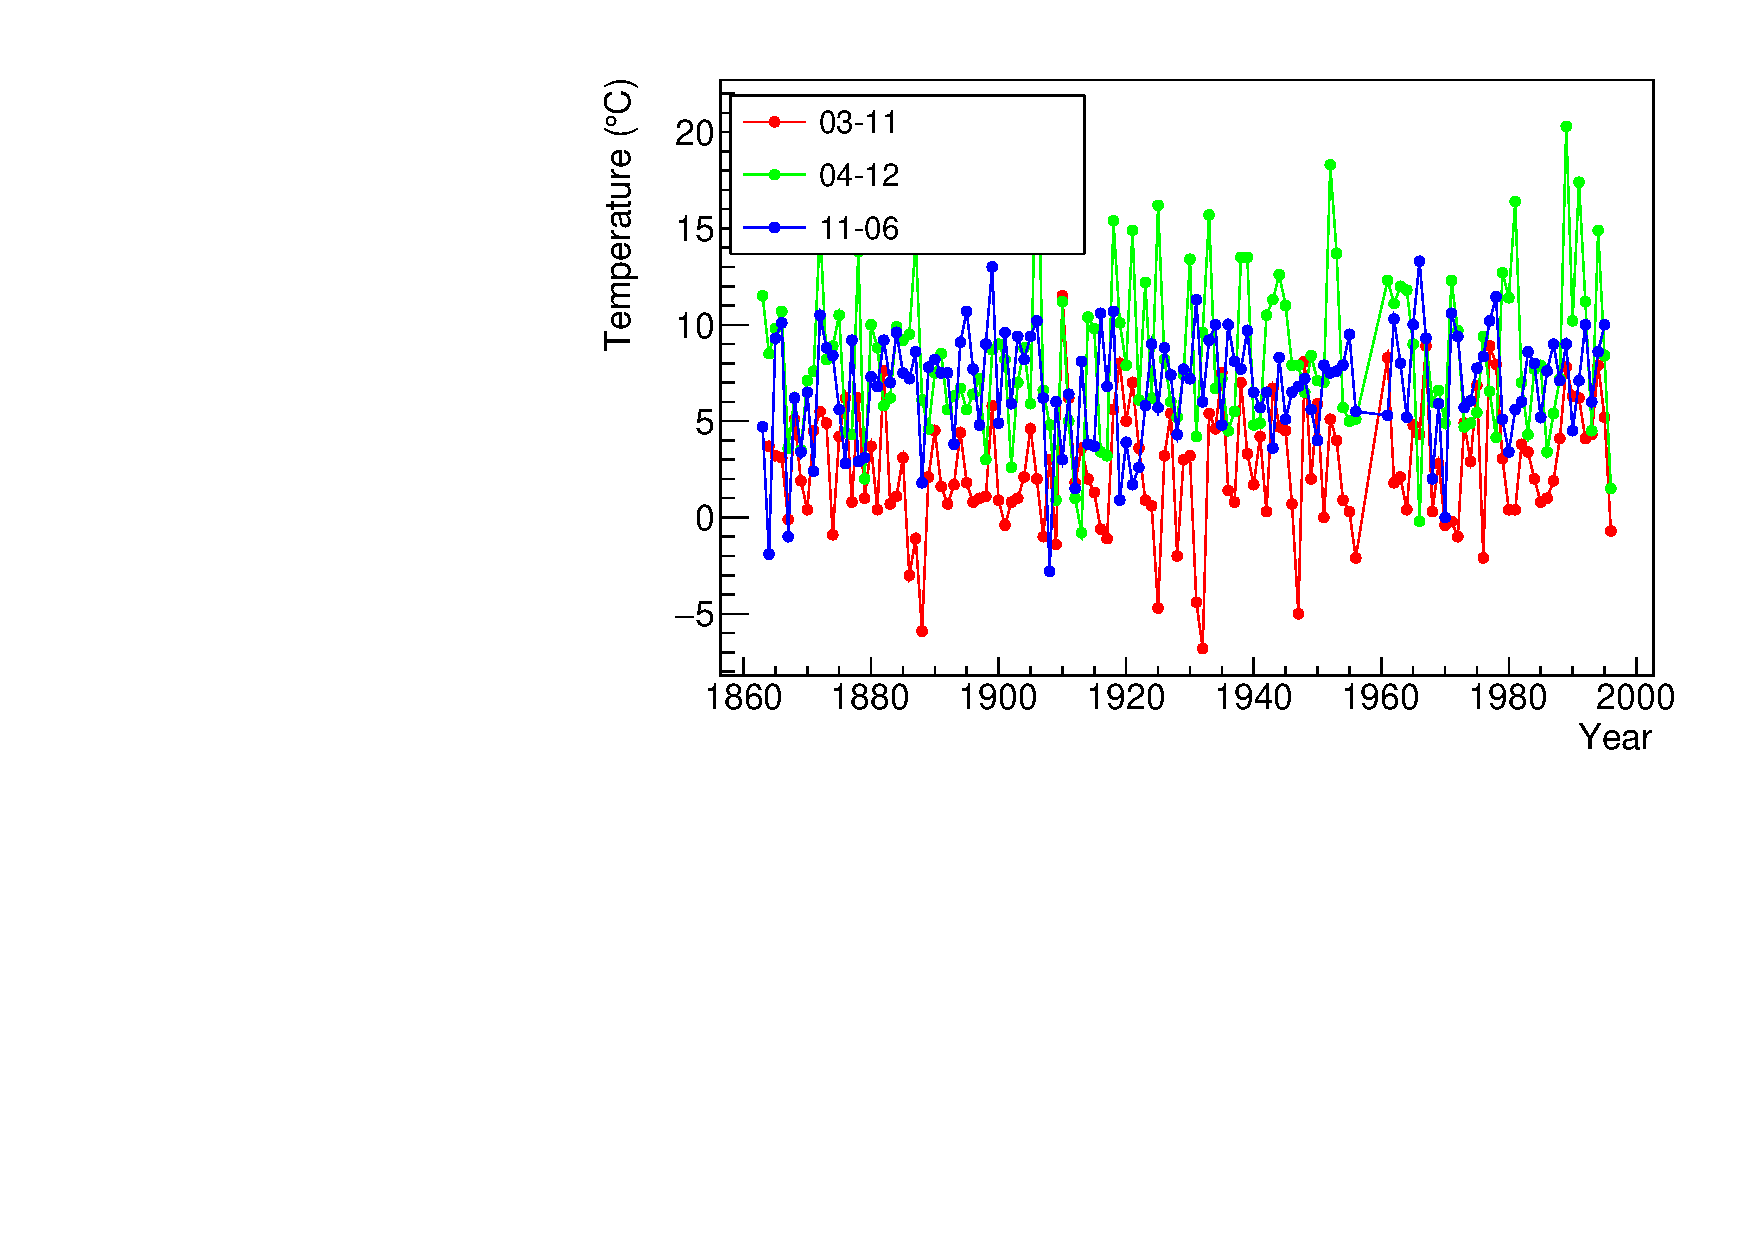
\includegraphics[width=0.85\linewidth]{../plots/bdays/Lundbdays.pdf}
    \caption{Average temperatures of the days 6/11, 12/4 and 11/3 between the years 1860 and 2000. The data was collected in Lund. The different days are labeled with different colors.}
    \label{fig:lund}
\end{figure}


\begin{figure}[H]
    \centering
    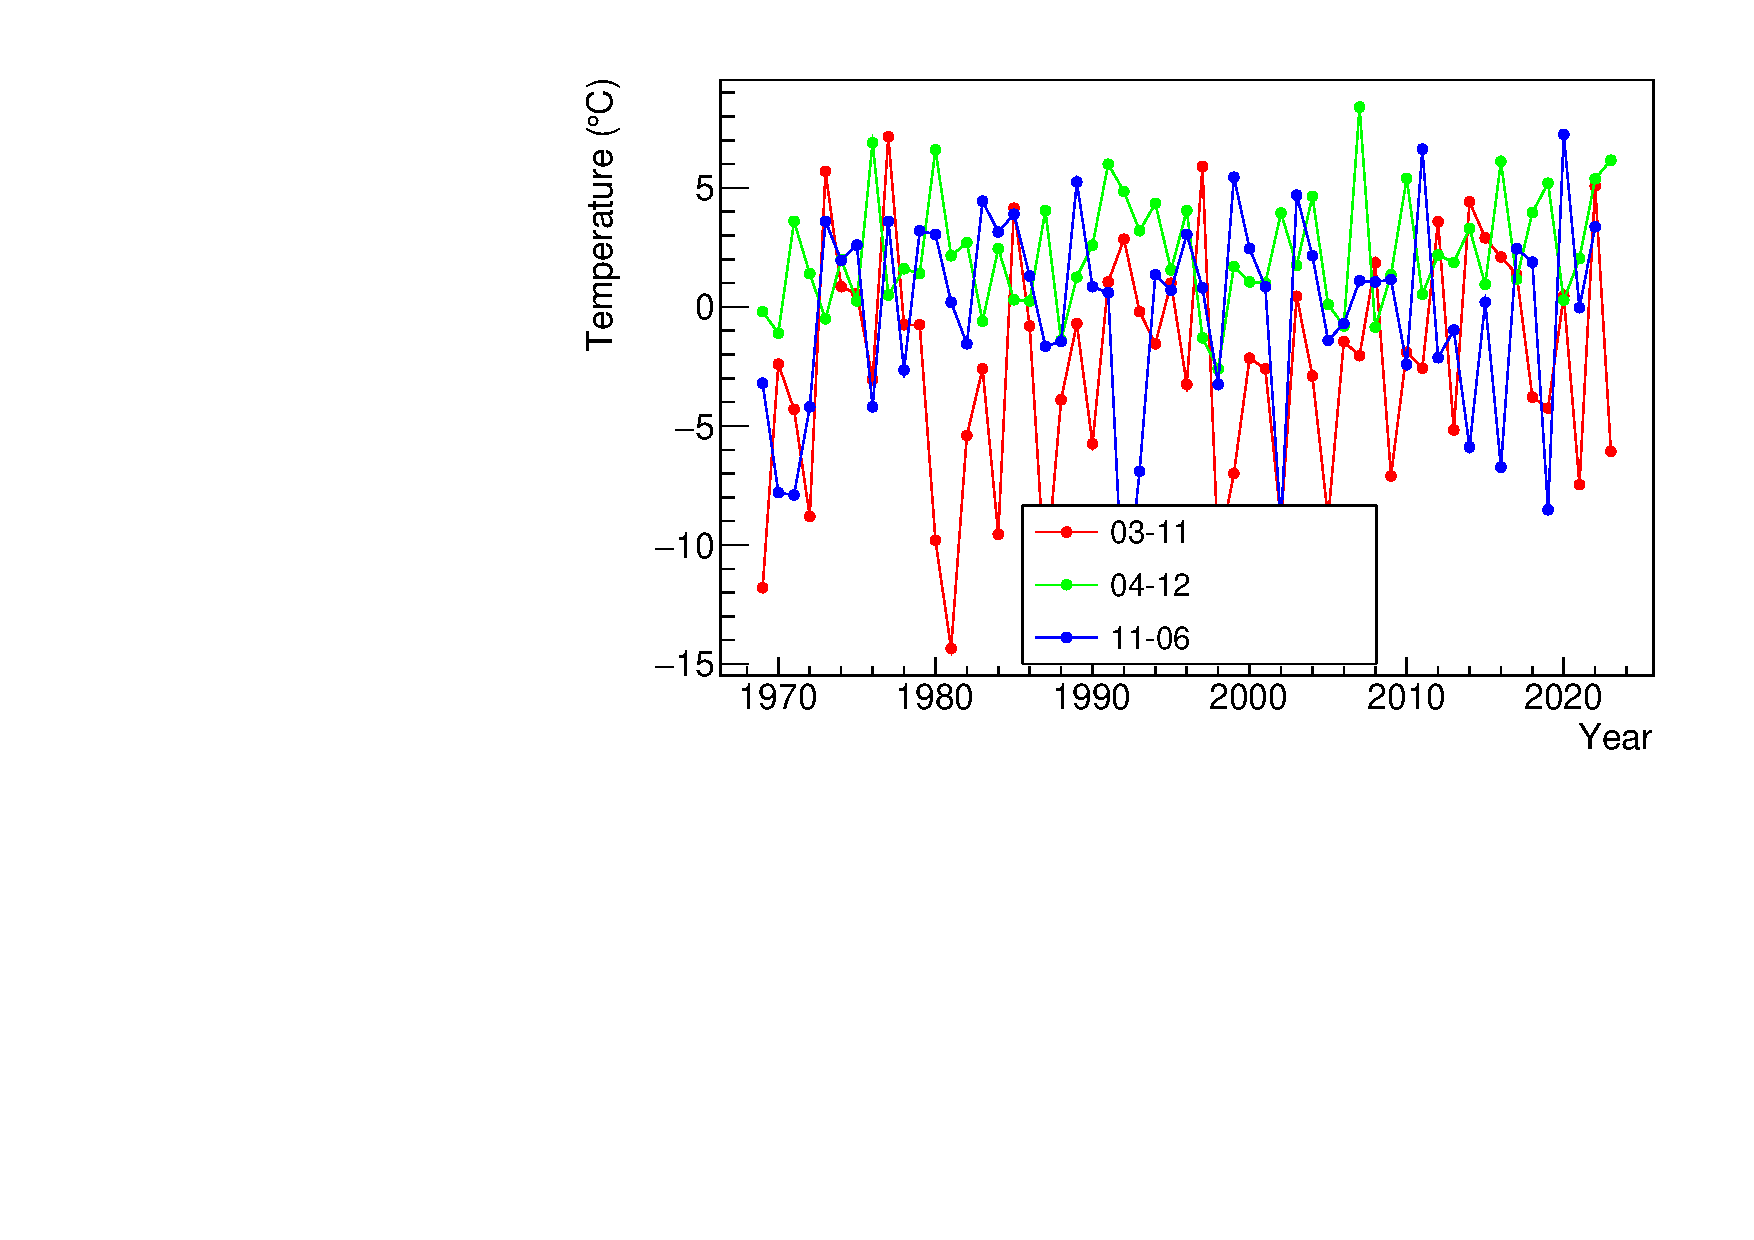
\includegraphics[width=0.85\linewidth]{../plots/bdays/Luleabdays.pdf}
    \caption{Average temperatures of the days 6/11, 12/4 and 11/3 between the years 1970 and 2025. The data was collected in Luleå. The different days are labeled with different colors.}
    \label{fig:luleå}
\end{figure}


\subsection{Discussion}
Figure \ref{fig:lund} and Figure \ref{fig:luleå} give multiple results that are worth discussing. The first result is that the average temperature each day changes in the same way each year, which is expected within the same city. However, which day that has the largest temperature change depends on the city. In Lund, the temperature seems to change the most in April and the least in November. In Luleå, it is the temperature in March that varies the most and in April it varies the least. The second clear result is that the average temperature for a specific day does not change a significant amount more than another. On temperatures all seem to increase a little bit over the years, which is expected. From another perspective, the average temperature in March and November seems to vary less during the last 15 years in Lund. The same can not be seen in Luleå but it is important to notice that the data only goes back to 1970 in Luleå. This is due to the filtering of the data before analyzing it, causing some years to not be included. This is something to consider to improve if the analysis is repeated in the future. One idea could be to have different analyses and results for different hours of the day. 

\subsection{Conclusion}
In conclusion, the analysis of the average temperature on our birthdays show no unexpected behaviour for any of the day. The variations in temperature stay consistent in each city and the recorded temperatures are expected. Both cities show a slow increase in average temperature but only Lund show less variation in temperature, especially in March and November. An important future improvement is to include the same amount of data points from each city to get a more accurate comparison. 
